\newcommand{\nom}{Porte conteneur}
\newcommand{\sequence}{03}
\newcommand{\num}{04}
\newcommand{\type}{TD}
\newcommand{\descrip}{Résolution d'un problème en utilisant des méthodes algorithmiques}
\newcommand{\competences}{Alt-C3: Concevoir un algorithme répondant à un problème précisément posé}
\documentclass[10pt,a4paper]{article}
  \usepackage[french]{babel}
  \usepackage[utf8]{inputenc}
  \usepackage[T1]{fontenc}
  \usepackage{xcolor}
  \usepackage[]{graphicx}
  \usepackage{makeidx}
  \usepackage{textcomp}
  \usepackage{amsmath}
  \usepackage{amssymb}
  \usepackage{stmaryrd}
  \usepackage{fancyhdr}
  \usepackage{lettrine}
  \usepackage{calc}
  \usepackage{boxedminipage}
  \usepackage[french,onelanguage, boxruled,linesnumbered]{algorithm2e}
  \usepackage[colorlinks=false,pdftex]{hyperref}
  \usepackage{minted}
  \usepackage{url}
  \usepackage[locale=FR]{siunitx}
  \usepackage{multicol}
  \usepackage{tikz}
  \makeindex

  %\graphicspath{{../Images/}}

%  \renewcommand\listingscaption{Programme}

  %\renewcommand{\thechapter}{\Alph{chapter}}
  \renewcommand{\thesection}{\Roman{section}}
  %\newcommand{\inter}{\vspace{0.5cm}%
  %\noindent }
  %\newcommand{\unite}{\ \textrm}
  \newcommand{\ud}{\mathrm{d}}
  \newcommand{\vect}{\overrightarrow}
  %\newcommand{\ch}{\mathrm{ch}} % cosinus hyperbolique
  %\newcommand{\sh}{\mathrm{sh}} % sinus hyperbolique

  \textwidth 160mm
  \textheight 250mm
  \hoffset=-1.70cm
  \voffset=-1.5cm
  \parindent=0cm

  \pagestyle{fancy}
  \fancyhead[L]{\bfseries {\large PTSI -- Dorian}}
  \fancyhead[C]{\bfseries{{\type} \no \numero}}
  \fancyhead[R]{\bfseries{\large Informatique}}
  \fancyfoot[C]{\thepage}
  \fancyfoot[L]{\footnotesize R. Costadoat, C. Darreye}
  \fancyfoot[R]{\small \today}
  
  \definecolor{bg}{rgb}{0.9,0.9,0.9}
  
  
  % macro Juliette
  
\usepackage{comment}   
\usepackage{amsthm}  
\theoremstyle{definition}
\newtheorem{exercice}{Exercice}
\newtheorem*{rappel}{Rappel}
\newtheorem*{remark}{Remarque}
\newtheorem*{defn}{Définition}
\newtheorem*{ppe}{Propriété}
\newtheorem{solution}{Solution}

\newcounter{num_quest} \setcounter{num_quest}{0}
\newcounter{num_rep} \setcounter{num_rep}{0}
\newcounter{num_cor} \setcounter{num_cor}{0}

\newcommand{\question}[1]{\refstepcounter{num_quest}\par
~\ \\ \parbox[t][][t]{0.15\linewidth}{\textbf{Question \arabic{num_quest}}}\parbox[t][][t]{0.85\linewidth}{#1\label{q\the\value{num_quest}}}\par
~\ \\}

\newcommand{\reponse}[4][1]
{\noindent
\rule{\linewidth}{.5pt}\\
\textbf{Question\ifthenelse{#1>1}{s}{} \multido{}{#1}{%
\refstepcounter{num_rep}\ref{q\the\value{num_rep}} }:} ~\ \\
\ifdef{\public}{#3 ~\ \\ \feuilleDR{#2}}{#4}
}

\newcommand{\cor}
{\refstepcounter{num_cor}
\noindent
\rule{\linewidth}{.5pt}
\textbf{Question \arabic{num_cor}:} \\
}

%%\usepackage[a4paper]{geometry}
%\geometry{margin={1cm,1.2cm}}
%\usepackage[francais]{babel}
%\usepackage{nopageno} %pas de numérotation de page
%\pagestyle{plain} %numérotation en bas de page, pas d'entête
%\usepackage{hyperref}
%\usepackage[latin1]{inputenc}

%%%%%%%%%%%%%%%%%%%%%%%%%%%%%%%%%%%%%%%%%%%%%%%%%%%%%%%%%%%%%%%%%%%%%%%%%%%%%%%%%%%%%

\usepackage{amsthm}
\usepackage{amscd}
%\usepackage{mathrsfs}
%\usepackage{amsfonts}
%\usepackage[T1]{fontenc}
%\usepackage{theorem}
\usepackage{lscape}
\usepackage{variations}  % pour faire des tableaux de variations
\usepackage{dsfont}
\usepackage{fancyvrb} % pour mettre Verbatim dans une box

% Pour les figures
\usepackage{subfig}
%\usepackage{calc} % Pour pouvoir donner des formules dans les d�finitions de longueur
%\usepackage{graphicx} % Pour inclure des graphiques 
% Attention : pour inclure des .jpg comme dans l'exemple (ou des .png ou .pdf)
% il faut compiler directement en pdf (commande pdflatex).
% Pour inclure des .eps, il faut compiler avec latex + dvips + ps2pdf.
\usepackage{psfrag}
%\usepackage{color}

%%%%%%%%%%%%%%%%%%%%%%%%%%%%%%%%%%%%%%%%%%%%%%%%%%%%%%%%%%%%%%%%%%%%%%%%%%%%%%%%%%%%%

\theoremstyle{definition}
\newtheorem*{thm}{Théorème}
%\theorembodyfont{\rmfamily}
\newtheorem*{defn}{Définition}
\newtheorem{exercice}{Exercice}
\newtheorem*{problem}{Problème}
\newtheorem*{prop}{Proposition}
\newtheorem*{corollaire}{Corollaire}
\newtheorem*{lemme}{Lemme}
\newtheorem*{remark}{Remarque}
\newtheorem*{notation}{Notation}
\newtheorem*{ex}{Exemple}
\newtheorem*{ppe}{Propriété}
\newtheorem*{meth}{Méthode}
\newtheorem*{rappel}{Rappel}
\newtheorem*{voca}{Vocabulaire}
\setlength{\columnseprule}{0.5pt}


%%%%%%%%%%%%%%%%%%%%%%%%%%%%%%%%%%%%%%%%%%%%%%%%%%%%%%%%%%%%%%%%%%%%%%%%%%%%%%%%%%%%%

\newcommand{\bi}{\bigskip}
\newcommand{\dsp}{\displaystyle}
\newcommand{\noi}{\noindent}
\newcommand{\ov}{\overline}
\newcommand{\dsum}{\displaystyle \sum}
\newcommand{\dprod}{\displaystyle \prod}
\newcommand{\dint}{\displaystyle \int}
\newcommand{\dlim}{\displaystyle \lim}

%%%%%%%%%%%%%%%%%%%%%%%%%%%%%%%%%%%%%%%%%%%%%%%%%%%%%%%%%%%%%%%%%%%%%%%%%%%%%%%%%%%%%


%\newcommand{\pgcd}{\mathrm{pgcd}} % pgcd
%\providecommand{\norm}[1]{\lVert#1\rVert} % norme
%\DeclareMathOperator{\Tan}{Tan}  % espace tangent


\newcommand{\N}{\mathbb{N}}
\newcommand{\Z}{\mathbb{Z}}
\newcommand{\Q}{\mathbb{Q}}
\newcommand{\R}{\mathbb{R}}
\newcommand{\C}{\mathbb{C}}
\newcommand{\K}{\mathbb{K}}
\newcommand{\U}{\mathbb{U}}
\newcommand{\Tr}{\text{Tr}\,}
\newcommand{\pg}{\geqslant}
\newcommand{\pp}{\leqslant}
\newcommand{\bul}{\item[$\bullet$]}
\newcommand{\card}{\text{Card}}
\newcommand{\re}{\text{Re}\;}
\newcommand{\im}{\text{Im}\;}
\newcommand{\Ker}{\text{Ker}\;}
\newcommand{\Vect}{\text{Vect}\;}
\newcommand{\rg}{\text{rg}\;}
\newcommand{\TT}{{}^t\!}
%\newcommand{\sh}{\text{sh}}
%\newcommand{\ch}{\text{ch}}
\newcommand{\Mat}{\text{Mat}}
\usepackage{textcomp}



%%%%%%%%%%%%%%%%%%%%%%%%%%%%%%%%%%%%%%%%%%%%%%%%%%%%%%%%%%%%%%%%%%%%%%%%%%%%%%%%%%%%%%%%%%%%%%%%%%%%%%%%%%%%%%%%%%%%%%%%%%%




\begin{document}

\begin{center}
{\Large\bf TP \no {\numero} -- \descrip}
\end{center}

\section{Connexion aux bases}

Ouvrir le logiciel MySQL Workbench (icône dauphin).

Si l'icône suivant apparaît cliquer dessus.

\begin{center}

\includegraphics[width=0.2\linewidth]{img/img01}
\end{center}

S'il n'apparaît pas, il faut configurer une nouvelle connexion en cliquant sur le bouton "+" et compléter les paramètres comme sur la figure ci-dessous. Une fois la connexion cinfigurée, il faudra préciser les mots de passe : \texttt{eleve} pour \texttt{eleve} et \texttt{b306} pour \texttt{dorian}.

\begin{center}
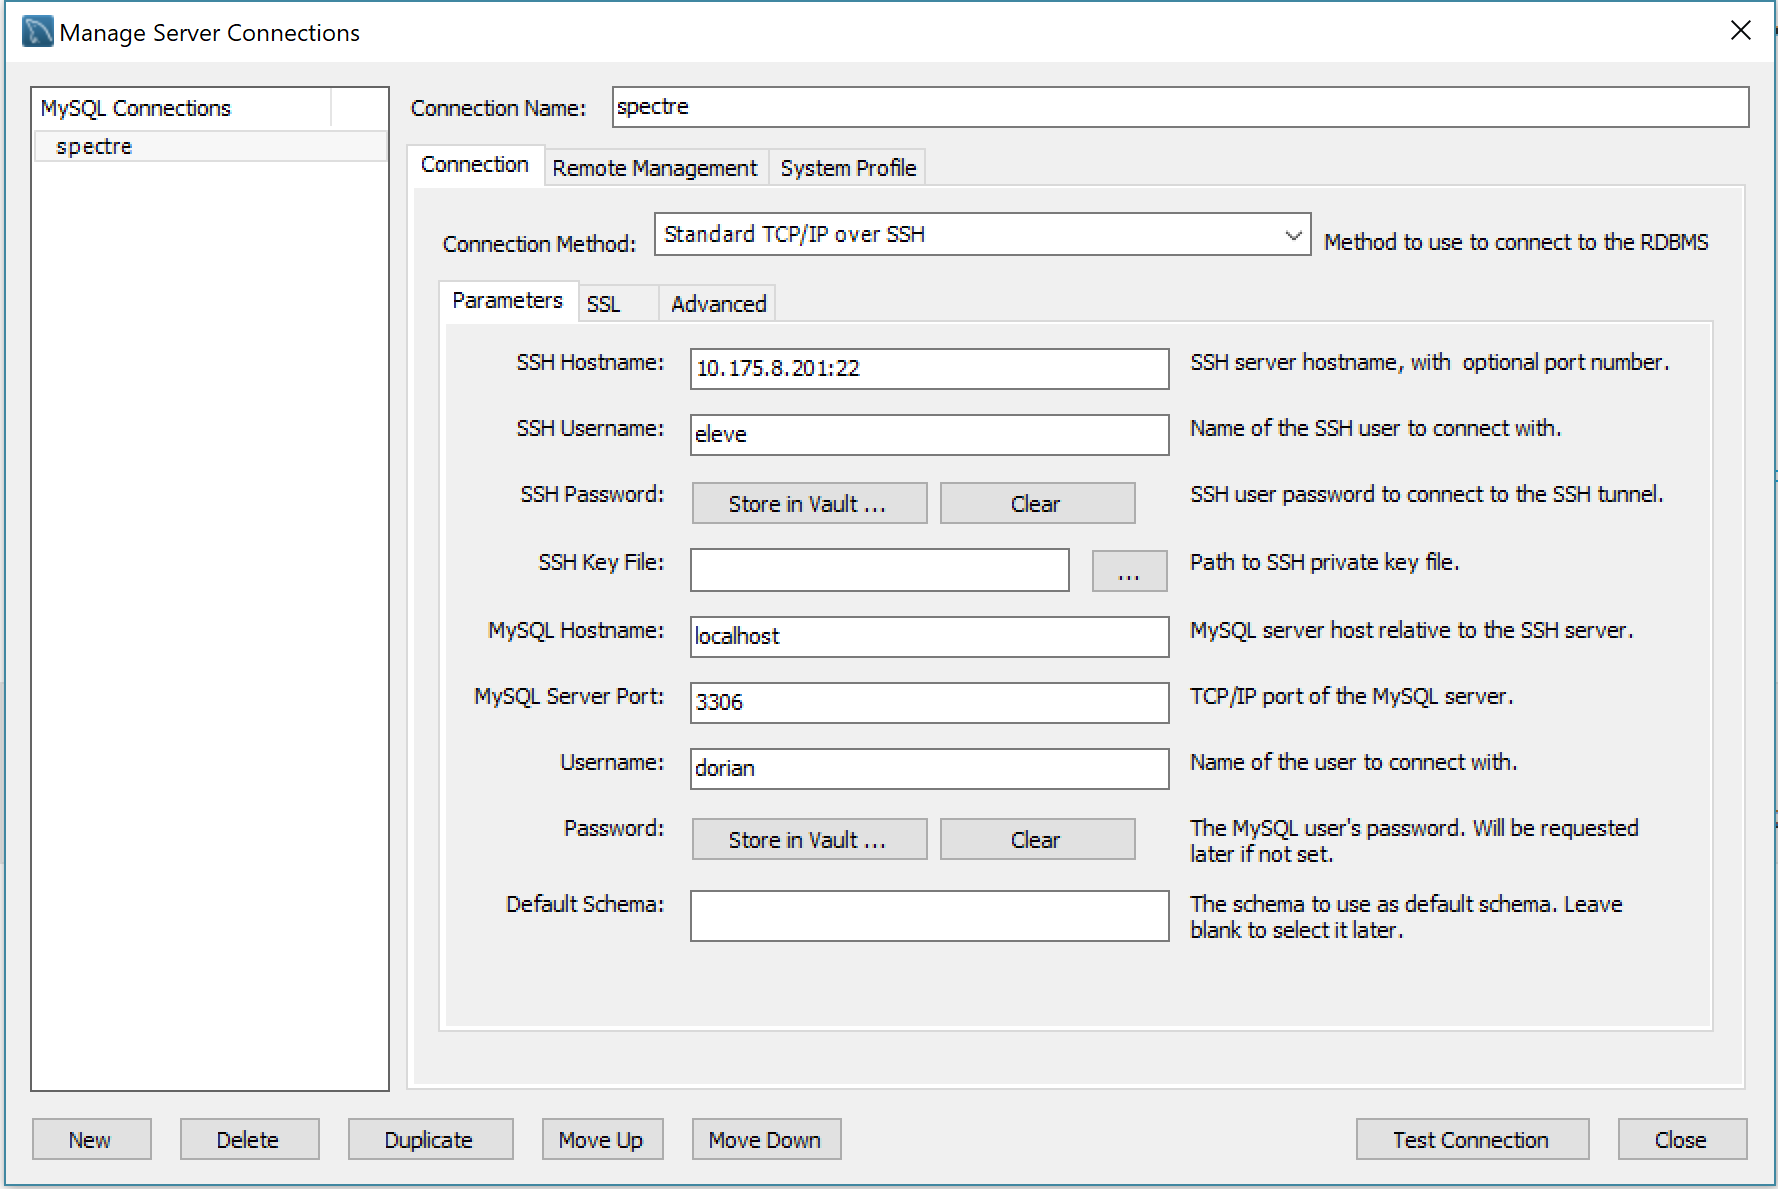
\includegraphics[width=0.8\linewidth]{img/img02}
\end{center}

Lorsque la nouvelle connexion a été configurée, l'icône mentionné précédemment apparaît, cliquer dessus.

\section{Triangles}

Double cliquer sur la base de données \verb|triangles| (colonne de gauche, \og SCHEMAS \fg) qui est une base de données constituée d'une seule table également nommées \verb|triangles| dont le schéma relationnel\footnote{Le schéma relationnel est le nom de la table, suivi des différents attributs et des domaines (entiers, texte, etc.) de ces attributs.} est le suivant : \verb|triangles  (idt:int, ab:int, ac:int, bc:int)|

Chaque ligne représente un triangle défini par la taille de ses trois côtés (AB, AC et BC).

\begin{enumerate}
 \item Après avoir réfléchi à leurs significations, lancer successivement les requêtes suivantes :
    \begin{itemize}
	\item[] \verb|SELECT COUNT(*) FROM triangles| ;
	\item[] \verb|SELECT * FROM triangles WHERE ab+ac+bc=100| ;
	\item[] \verb|SELECT ab*ac*bc FROM triangles WHERE ab+ac+bc>=100| ;
    \end{itemize}

 \item Déterminer à l'aide de requêtes SQL :
 
    \begin{enumerate}
      \item la plus petite valeur des produits AB x AC x BC pour les triangles ABC de périmètre supérieur ou égal à 100 ;
      \item les longueurs AB, AC et BC correspondants aux triangles pour les lesquels le minimum précédent est atteint ;
      \item tous les triangles rectangles en A ;
      \item le nombre de triangles rectangles en A ;
      \item le maximum des périmètres des triangles rectangles en A ;
      \item tous les triangles équilatéraux ;
      \item tous les triangles tels que $\frac{AB+AC+BC}{3} = 42$
      \item exporter\footnote{Une des « actions » au dessus des résultats de la requête est faite pour cela.} les résultats de la requête précédente dans un fichier au format csv.
    \end{enumerate}

\end{enumerate}

\section{Communes, département et régions}

\begin{enumerate}
 \item Ouvrir la base de données \verb|communes| en double cliquant dessus et écrire sur papier les schémas relationnels des trois tables qu'elle contient. On obtient le schéma relationnel d'une table en sélectionnant cette table dans la barre latérale gauche puis en cliquant sur l'onglet « Object Info ».
 
 \item Exécuter la requête suivante :
 
 \verb|SELECT communes.nom, departements.nom|\\
 \verb|FROM communes JOIN departements|\\
 \verb|ON communes.dep=departements.id|

 Pour simplifier l'écriture de telles requêtes, on peut utiliser des alias pour chacune des tables, grâce à l'opérateur \verb|AS|. Par exemple, la requête précédente peut s'écrire :
 
 \verb|SELECT C.nom, D.nom FROM communes AS C JOIN departements AS D ON C.dep=D.id|
 
 \item En vous inspirant du modèle précédent, déterminer la liste de toutes les communes avec pour chacune son département, sa région et sa population.
 
\item \begin{enumerate}
\item Déterminer la liste des villes de plus de cent milles habitants avec leur population et leur région.                                                                                                    
\item Trier la liste précédente par ordre décroissant de population. On pourra pour cela utiliser la commande \verb|ORDER BY| (voir Annexe).
\end{enumerate}

\item Déterminer la liste des communes (nom et population) dont le nom commence par \verb|Pa| et se termine par \verb|is|. On pourra pour cela utiliser l'opérateur \verb|LIKE| (voir Annexe).

\item Déterminer les communes dont le nom a strictement plus de lettres que leur nombre d'habitants. On pourra utiliser la fonction \verb|LENGTH| (voir Annexe).
\end{enumerate}


\section{Création et alimentation d'une base de données}
\subsection{Organisation d'une base de données}

\begin{enumerate}
  \item Ouvrir la base de données nommée \verb|eleves|. 
  \item Créer une table dont le schéma relationnel est le suivant :

  \verb|films_nom_prenom (titre:text, realisateur:text, annee:int)| (en remplaçant nom et prenom par \textbf{votre} nom et \textbf{votre} prénom)
   
  \item Ajouter des entrées à la table, à partir des informations fournies en Annexe. Consignes : l'attribut \verb|realisateur| ne doit contenir qu'un seul nom et toutes les informations doivent être présentes dans la table.

  \item La table précédente contient plusieurs fois des informations strictement identiques. Rechercher par exemple l'année de sortie du film \textit{Sacré Graal}.
  
  \item En vous inspirant de la deuxième partie du TP, déterminer comment modifier la table \verb|films_nom_prenom| et quelle autre table créer (toujours avec vos nom et prénom comme suffixes) pour éviter les informations en doublons.
  
  \item Mettre en œuvre une solution et effectuer une requête sur une jonction des deux tables permettant d'obtenir les noms des réalisateurs du film \textit{Sacré Graal}.
\end{enumerate}

\subsection{Exploitation d'une base de données}

Le contenu de la table \verb|cafes| vient de la liste\footnote{Récupérée sur http://opendata.paris.fr} des noms, des adresses et des coordonnées géographiques des endroits de Paris où le café était servi à 1 euro au 15 mai 2014.

\begin{enumerate}
 \item Combien de cafés sont situés dans le XI\up{e} arrondissement ?
 
 \item Les coordonnées géographiques du lycée Dorian sont en degrés décimaux : (latitude) 48,854563° et (longitude) 2,392678°. Pour des lieux tous situés dans une zone géographique aussi petite que Paris, on peut approximer que la distance entre deux points est directement proportionnelle à la racine carrée de la somme de la différence des longitudes au carré et de la différence des latitudes au carré : $\sqrt{(lat1-lat2)^2  + (long1-long2)^2}$. Quel est le café à un euro le plus proche du lycée ?
\end{enumerate}

\section{Utilisation de bases de données avec Python (Optionnel)}

\begin{enumerate}
  \item Ouvrir un nouvel éditeur de script IDLE. Enregistrer votre fichier de script dans votre répertoire personnel. Taper dans le script les lignes suivantes :

  \begin{minted}[linenos,frame=lines]{python}
  import MySQLdb
  base = MySQLdb.connect (host = '10.175.8.201',
                        user = 'dorian',
                        passwd = 'dorian',
                        db = 'triangles')
  curseur = base.cursor ()
  res = curseur.execute("""SELECT * FROM triangles WHERE ab+ac+bc=100""")
  foo = curseur.fetchall()
  base.close()
  \end{minted}

  \item Quels types d'objets Python sont \verb|res| et \verb|foo| ? Que contient \verb|foo| ?

  \item À l'aide d'une requête effectuée depuis le script Python, déterminer les triangles tels que $\frac{AB+AC+BC}{3} = 42$ et placer les résultats dans un fichier. Comparer avec la méthode n'utilisant que SQLite Manager (dernière question de l'exercice 1).
\end{enumerate}

\newpage
\section{Annexe}
\subsection{ORDER BY}

La clause \verb|ORDER BY attribut| permet de trier les résultats de la requête selon un attribut donné. Par défaut le tri est ascendant. L'option \verb|DESC| permet de trier par ordre descendant.

\verb|ORDER BY nom| trie la requête par ordre ascendant des valeurs de l'attribut \verb|nom|

\verb|ORDER BY annee DESC| trie la requête par ordre descendant des valeurs de l'attribut \verb|annee|

Elle est toujours située à la fin de la requête.

\subsection{LIKE}

L'opérateur \verb|LIKE|, utilisé en complément de la clause \verb|WHERE| permet de sélectionner sur la base d'un modèle (par exemple, la valeur de l'attribut commence/se termine ou comprend une séquence de caractères particulières, le « modèle »). 

Syntaxe : \verb|SELECT * FROM table WHERE attribut LIKE modele|

Modèle : le modèle est une chaîne de caractères, contenue entre guillemets, avec comme caractère joker le caractère « \% ». 

Exemples :
\verb|LIKE "%a"| : permet de rechercher toutes les chaînes de caractère qui se termine par un « a ».\\
\verb|LIKE "a%"| : permet de rechercher celles qui commencent par un « a ».\\
\verb|LIKE "%a%"| : pour rechercher celles qui utilisent le caractère « a ».\\
\verb|LIKE "pa%on"| : permet de rechercher les chaînes qui commencent par « pa » et qui se terminent par « on », comme « pantalon » ou « pardon ».

\subsection{LENGTH}

La fonction \verb|LENGTH| renvoie la longueur d'une chaîne de caractères. 

\verb|LENGTH("total")| renvoie \verb|5|.

Utilisée sur un attribut avec la clause \verb|WHERE|, elle permet de faire des recherches avec comme critère la longueur d'un attribut de type texte ou chaîne de caractères.

\subsection{Liste de films}
Voici trois films, suivi du ou des réalisateurs et de l'année de sortie.

\begin{itemize}
 \item \textit{Sacré Graal} de Terry Jones et Terry Gilliam sorti en 1975.
 \item \textit{La Vie de Brian} de Terry Jones sorti en 1979.
 \item \textit{Brazil} de Terry Gilliam sorti en 1985.
\end{itemize}

\end{document}
